\documentclass[10pt,twocolumn,letterpaper]{article}

\usepackage{cvpr}
\usepackage{times}
\usepackage{epsfig}
\usepackage{graphicx}
\usepackage{amsmath}
\usepackage{amssymb}

% Include other packages here, before hyperref.

% If you comment hyperref and then uncomment it, you should delete
% egpaper.aux before re-running latex.  (Or just hit 'q' on the first latex
% run, let it finish, and you should be clear).
\usepackage[breaklinks=true,bookmarks=false]{hyperref}
\usepackage[utf8]{inputenc}

\cvprfinalcopy % *** Uncomment this line for the final submission

\def\cvprPaperID{****} % *** Enter the CVPR Paper ID here
\def\httilde{\mbox{\tt\raisebox{-.5ex}{\symbol{126}}}}

% Pages are numbered in submission mode, and unnumbered in camera-ready
%\ifcvprfinal\pagestyle{empty}\fi
\setcounter{page}{4321}
\begin{document}

%%%%%%%%% TITLE
\title{Computer Vision Lab 05 -Segmentations BSD500}

\author{Juan Carlos Leon Alcazar\\
Universidad de los Andes\\
{\tt\small jc.leon@uniandes.edu.co}
% For a paper whose authors are all at the same institution,
% omit the following lines up until the closing ``}''.
% Additional authors and addresses can be added with ``\and'',
% just like the second author.
% To save space, use either the email address or home page, not both
\and
\\
\\
\\
{\tt\small }
}

\maketitle
%\thispagestyle{empty}


\section{Description of the database}

The database\cite{Lazebnik2005} contains 1000 gray scale in JPG format, all of them have a standard 640x480 pixels resolution. Images are close ups of a given object surface, thus, containing textures found in different objects. There is a total of 17 classes \footnote{The object classes are: Bark Wood, Water, Granite, Marble, Floors, Pebbles, Wall Brick, Glass, Carpet, Upholstery, Wallpaper, Fur, Knit, Corduroy \& Plaid }, each contains between 30 to 90 sample images in the train set and between 10 to 30 images in the test set. Finally, there is a plain text file which specifies the naming convention for the images.


\section{Methodlogy}

the overall methodology used in this laboratory is presented in figure \ref{fig:pipeline}. Initially a texton filter bank is created and then used to create a texton dictionary is over a subset of randomly subsampled images from the training set. With this dictionary the texton responses of the test set are calculated, such responses are used to characterize the textures on the test set with a Nearest Neighbour (NN) classifier or a Random Forest classifier.

\begin{figure*}
\begin{center}
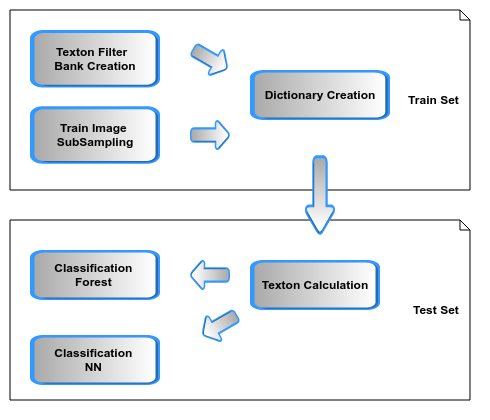
\includegraphics[width=0.65\textwidth]{img/Pipeline.png}
\end{center}
\caption{Elements of the proposed apporach}
\label{fig:pipeline}
\end{figure*}

\subsection{Train Set Subsample}
The original first step in the pipeline was the construction of a texton dictionary from the whole train subset.  However, due to hardware constraints, it was not possible to build this dictionary with the complete train set (750 images). Creating a texton dictionary with a set of 40 images already requires about 45 GB of RAM memory (At peak), and about 3 hours CPU time. For the experiments, a single 115GB RAM machine was available. As it was not possible to create a dictionary with the full training set, it was reduced to 170 images (10 images per class).

There is not a clear way to subsample the original training set while retaining the original data variability, in other words, it is expected that this sub sampling process should create some bias in the dictionary. However the nature of the dataset might help to mitigate this issue: textures are essentially local patterns repeated, with some variability, at the global level. Thus it can be assumed that each image contains several instances of these local patterns, that already contain some of the variability of the texture.

\subsection{Texton Filter Bank}
At the very beginning of this processing pipeline it is very hard to predict which filter bank will have better performance  on the classification step, therefore the default set of filters is used. This set contains 16 filters a two differents scales. Within a given scale filters follow approximately the same spatial pattern and vary mostly on their orientation. Figure \ref{fig:FB} show a sample of the textons used.

\begin{figure}


\includegraphics[width=0.95\linewidth]{img/FilterBank.png}
\begin{center}
\caption{The texton filter bank used (single scale)}
\end{center}
\label{fig:FB}
\end{figure}


\subsection{Texton Dictionary Creation}
After selecting the initial number of training images, there remains one final parameter for the construction of the texton dictionary, namely the K for the K means. For this matter we use a number of textons given by $K=c32$ ($c={1,2,3}$). The explanation behind this choice is that we expected the local patterns to closely match the shape of the filter bank; This is the case of c=1 $\rightarrow$ K=32. However, not every local pattern will match perfectly one of the textons on the filterbank. This is the case of $K={2,3}$ where the resulting clusters might contain the response information of several filters. No further values for $c$ are explored mostly, due to time constraints.
The final setup for the texton dictionary construction is the following:

\begin{itemize}
	\item Filter Bank: default filterbank provide in the implementations 16 orientations, 2 scales
	\item Number of training images: 170 (10 per class)
	\item Number of clusters ($N$):  32, 64, 96
\end{itemize}

\subsection{Texton Calculation on Test Set}

With the 3 Texton dictionaries built we then calculate response of every image in the test set filtered with the obtained textons. for each image we obtain 3 responses (3 dictionaries) which are then represented by means of an histogram where the number of bins depends on the value of K used for the construction of the dictionary.

\subsection{Classification}
There are two methods selected for the classification of the textures

\begin{description}

\item[Nearest Neighbor] The  Nearest Neighbor (NN) algorithm is built upon an arbitrary distance metric among the training set, a new object is given a label based on its closest neighboring objects \cite{Gorunescu2011}
\item[Random Forest] A random fortes is an ensemble of classifiers, each of them follows a tree like structure where each node is a weak learner that tries to maximize the information gain. Each node then create a split in the data over a subset of the data dimensions available at that node\cite{Liaw2002}

\end{description}

The first methods has a single parameter: the distance metric, as specified by the assignment, we use the Chi-square distance to choose the NN..

For the second method there are more parameters, the MATLAB implementation allows to choose:

\begin{itemize}
	\item Number of variables eligible for each decision split
	\item Cost of misclassifications
	\item Minimum number of observations per tree leaf
\end{itemize}

To allow for a maximum variability in the built trees we select the number of variables eligible for each decision split equals to the total amount of variables. Set the minimum number of observations to 1 and set no specific cost matrix for the experiments.

No other adjustment is performed on the test data or the texton dictionary after being calculated.

\section{Results}
Tables \ref{table:table1} and \ref{table:table2}  summarize the results obtained for the NN and the Random Forest classifier:

\begin{table*}[t]
\centering
\begin{tabular}{c | c | c}
Set Up & Precision & Recall   \\
\hline	
K=32 & 0.072 & 0.094 \\
K=64 & 0.1609 & 0.4667 \\
K=96 &  0.1163&  0.2553 \\

\end{tabular}
\caption{Precision and recall for the Nearest neighbor classifier}
\label{table:table1}
\end{table*}


\begin{table*}[t]
\centering
\begin{tabular}{ l | c | c}
Set Up & Precision & Recall   \\
\hline	
K=32,20 trees & 0.1159 & 0.2667 \\
K=64,20 trees & 0.1552 & 0.3000 \\
K=96,20 trees & 0.0789  &  0.2000 \\
K=32,50 trees & 0.1585 & 0.4333 \\
K=64,50 trees & 0.1458 & 0.3333 \\
K=96,50 trees &  0.1111 &  0.2333\\
K=32,100 trees & 0.1477 & 0.4333  \\
K=64,100 trees & 0.1687 & 0.4667  \\
K=96,100 trees & 0.1609 &  0.4667\\
K=32,500 trees & 0.1638 & 0.6333  \\
K=64,500 trees & 0.2072  &  0.7667 \\
K=96,500 trees & 0.1475 & 0.6000  \\

\end{tabular}
\caption{Precision and recall for the Random Forest classifier}
\label{table:table2}
\end{table*}


Overall both classifiers perform very poorly on the test set. The Nearest Neighbour classifier for K=32 has a performance slightly better than that of a random guess over the set of 17 classes. This behavior suggest that for K=32 the inter-class distances in the test set are very small and that the class distribution does not follow an approximate cluster pattern in the space generated by the chi-square distance metric. As result it is very hard for any classifier to separate the classes.

For K=64 the results are similar for both classifiers yet they barely reach a 0.2 precision. This figure suggest that both classifiers underperform mostly due to a very high number of false positives. This can be further confirmed in table \ref{table:table4} which presents the confusion matrix for the best classifier found in this laboratory (Random Forest classifier K=64, 500 trees). It has a strong tendency to classify samples as belonging to classes bark and wood, it mostly ignores every other class.

With the current experimental setup, this tendency to misclassify the data can be due to:

\begin{itemize}
	\item Errors during training phase
	\item Selected training data does not approximate the actual variability of the test data (underfitting)
\end{itemize}

To better establish the source of error, we train and classify over the same subset (test). This experimental setup yields a precision of 1.0 and recall of 1.0 for the random forest with K=32. The obvious overfit scenario rules out possible errors during the training phase and further in indicates that: while the classifier can learn the patterns over the training set, \textbf{the patterns at the training set are not discriminative enough to properly classify the test set}

This situation can be attributed mostly to the subsampling made on the training set, 10 samples per class is not enough to capture the complete variability of the textures.






\begin{table*}[t]
\centering
\tiny
\begin{tabular}{c | c | c |c |c |c |c |c |c |c |c |c |c |c |c |c |c | c | c }
& Bark & wood & Water & Granite & Marble & Floor & Pebbles & Wall & Brick1 & Glass1 & Carpet &upholstery &wallpaper & Fur &	knit & corduroy &	plaid \\
\hline	

Bark &	23   &  7 &    0 &    0   &  0   &  0  &   0 &    0   &  0    & 0   &  0  &   0  &   0 &    0  &   0 &    0  &   0\\
Water &   5   & 22   &  0  &   0   &  0   &  2   &  0   &  0   &  1   &  0   &  0  &   0  &   0  &   0  &   0  &   0  &   0\\
Wood &    3   &  3   &  0  &   0   &  0   &  1   &  0   &  0   &  3   &  0   &  0  &   0  &   0  &   0   &  0  &   0  &   0\\
Granite &  6   &  4   &  0  &   0   &  0   &  0   &  0   &  0   &  0   &  0   &  0  &   0  &   0  &   0   &  0  &   0  &   0\\
Marbel &   1   &  8   &  0  &   0   &  0   &  1   &  0   &  0   &  0   &  0   &  0  &   0  &   0  &   0   &  0  &   0  &   0\\
Floor &    5   & 14   &  0  &   0   &  0    & 0   &  0  &   0   &  1   &  0   &  0  &   0  &   0  &   0   &  0   &  0  &   0\\
Pebbles &  8   &  1   &  0  &   0   &  0    & 0  &   0  &   0   &  0   &  1   &  0  &   0  &   0  &   0   &  0 &    0   &  0\\
Wall &  1   &  8   &  0   &  0   &  0    & 0   &  0  &   0   &  1   &  0   &  0  &   0  &   0  &   0   &  0  &   0   &  0\\
Brick &   7   &  9   &  0   &  0   &  0    & 0   &  0   &  0   &  4   &  0   &  0  &   0  &   0  &   0   &  0  &   0   &  0\\
Glass &  15   &  3   &  0   &  0   &  0    & 1   &  0   &  0   &  0   &  0   &  1  &   0  &   0  &   0   &  0   &  0  &   0\\
Carpet &  17   &  3   &  0   &  0   &  0    & 0   &  0   &  0   &  0   &  0   &  0  &   0  &   0  &   0   &  0   &  0  &   0\\
Upholstery &   5   &  5    & 0   &  0   &  0   &  0   &  0   &  0   &  0   &  0   &  0  &   0  &   0  &   0   &  0   &  0   &  0\\
Wallpaper &   0   &  7   &  0   &  0   &  0   &  0   &  0   &  0   &  3   &  0   &  0  &   0  &   0  &   0   &  0   &  0   &  0\\
Fur &   3   &  6   &  0   &  0   &  0   &  0   &  0   &  0  &   0   &  1   &  0  &   0  &   0  &   0   &  0  &   0   &  0\\
Knit &  4   &  5   &  0   &  0   &  0   &  1   &  0   &  0  &   0   &  0   &  0  &   0  &   0  &   0   &  0  &   0   &  0\\
Corduroy &   6   & 2   &  0    & 0    & 0    & 0    & 0    & 0   &  1    & 1    & 0    & 0   &  0   &  0    & 0   &  0   &  0\\
Plaid &   2   &  7  &   0   &  0   &  0   &  0   &  0   &  0   &  1   &  0   &  0   &  0   &  0  &   0   &  0  &   0  &   0\\
\end{tabular}
\caption{Confusion matrix for the Random Forest classifier K=64, 500 trees}
\label{table:table4}
\end{table*}

\subsection{Training and execution times}
Table \ref{table:times} summarizes the training times for the Random forest classifier.

\begin{table*}[t]
\centering
\begin{tabular}{ l | c | c}
Setup & Training time (Seconds) & Classification time (Seconds)    \\
\hline	
K=32,20 trees & 35.11 & 0.042817\\
K=64,20 trees &   36.30 & 0.001 \\
K=96,20 trees &  33.21  & 0.001 \\
K=32,50 trees & 83.15  & 0.063 \\
K=64,50 trees &  86.37 & 0.092 \\
K=96,50 trees &   79.52 & 0.081 \\
K=32,100 trees &  167.52 & 0.161 \\
K=64,100 trees &  169.77 & 0.211 \\
K=96,100 trees &  162.20 & 0.161\\
K=32,500 trees &  794.10 & 0.811 \\
K=64,500 trees &  810.67 & 0.963 \\
K=96,500 trees &  769.05 & 0.801 \\

\end{tabular}
\caption{Training Time (seconds) for different configurations, times measured in a laptop computer with an Quad Core INTEL I7 and 12GB RAM}
\label{table:times}
\end{table*}

The training time is mostly not an issue for the Random Forest Classifier, as it can be completed usually in 2 minutes or less, the only exception are the cases where the amount of trees is greater than 100, where it takes about 13 minutes. It should also be noticed thet the K used to build the filter bank has little impact the total computation time. Unlike the filter dictionary calculation the training process requires very little RAM memory resources, usually under 400MB.


Overall classification is an extremely fast task, times are never over 1 second for the whole test set (250 images).


Table \ref{table:timesNN} summarizes the training times for NN classifier.

\begin{table*}[t]
\centering
\begin{tabular}{ l | c | c  }
Setup & Training time (Seconds) & Classification time (Seconds)    \\
\hline	
K=32 & 2.55& 5500 \\
K=64 & 2.52 & 5631  \\
K=96 & 3.11 &  4870 \\

\end{tabular}
\caption{Classification time (seconds) for different configurations of the NN classifier, times measured in a laptop computer with an Quad Core INTEL I7 and 12GB RAM}
\label{table:timesNN}
\end{table*}

Overall the training times are much smaller for the NN classifier (under 4 seconds in any case), but the classification process is much slower, this is probably due to the fact that the chi-square distance must be calculated for every sample in the test set (there are 750 samples in the training set).

\subsection{Method Limitations \& Improvements}
As mentioned earlier, the poor performance of the method seems to be related to the subsampling made to the train set. This is not a limitation of the method itself, but rather a hardware limitation.

The most important modification that could be made to the method is to develop a better  subsampling strategy for the the train set, where little  variability is lost.

One such strategy could be to densely sample patches over the whole training set, and create a subset,  by pruning similar or homogeneous patches . This pruning could be done by means of a similarity  metric, like a standard cross correlation, mutual information or even a learnt metric that can adapted to the different textures information on the dataset size.

A second approach  would be to first build a dictionary of a bag of visual word  for  every texture category and then train the texton dictionary only with those patches that are the most discriminative among the categories.

Finally, an obvious improvement, would be to re-implement the most relevant functions so that the memory usage during the dictionary construction phase is reduced and the initial texton dictionary can be built with a larger amount of images

\subsection{Database Limitations}
With such poor classifications results, that can be attributed to a sub optimal texton dictionary, it is hard to make any statement about the limitations of the database. Still, it would be interesting to have color images to add more information to the classification process; Scale information would also be useful to create better multi scale classification strategies.


\section{Extra Credit}
Given the poor results obtained in the firts version of the laboratory, the complete experimental setup was revisited for the extra credit actvities. The texton dictionary was calculated again with five random images from each class. Tree diffrent texton dictionaries where built for K=10,20,50. Every image not used in the dictionary construction was then represented with the dictionary and used in the learning process.

There are two initial taks related to the filter bank construction on extra credit. 

\begin{description}

\item[Another spatial scale] Can be directly achived by the code provided, just call the function  'fbCreate' with the argument 'numScales' set to 3. A short hadn function for this was created and reduced to 'fb=createBank(16,2);'

\item[Gaussian Filters] The gaussian filters can be created with the function 'fspecial', before the experiments it is not possible to establish which gaussian filtar can produce the best result so 6 filter are built for each scale with the standar deviatio ranging from 0.1 to 50 (see runTextonRepresentationGaussian.m)



\end{description}

The final step is the svm classifier. As outlined early in this section the representation of the test images is used to train a multi-class svm and the test set is used to evaluate the results. These are summarized in table \ref{}

\begin{table*}[t]
\centering
\begin{tabular}{ l | c | c  }
Setup & Precision & Recall    \\
\hline	
K=10 Extra Scale & 0.08 & 1  \\
K=20 Extra Scale & 0.08 & 1  \\
K=50 Extra Scale & 0.08 & 1  \\
K=10 Gaussian Filters & 0.08 & 1 \\
K=20 Gaussian Filters & 0.08 & 1 \\
K=50 Gaussian Filters & 0.08 & 1  \\

\end{tabular}
\caption{}
\label{table:extraPR}
\end{table*}


Training and classification times


\begin{table*}[t]
\centering
\begin{tabular}{ l | c | c  }
Setup & Training time (Seconds) & Classification time (Seconds)    \\
\hline	
K=10 Extra Scale & 346.38 & 17.59 \\
K=20 Extra Scale & 376.01 & 27.80 \\
K=50 Extra Scale & 433.94 &  26.04\\
K=10 Gaussian Filters & 287.58 & 35.00 \\
K=20 Gaussian Filters & 272.73 & 18.19 \\
K=50 Gaussian Filters & 256.83 & 17.52 \\


\end{tabular}
\caption{Classification time (seconds) for different configurations of the NN classifier, times measured in a laptop computer with an Quad Core INTEL I7 and 12GB RAM}
\label{table:timesNN}
\end{table*}


{\small
\bibliographystyle{ieee}
\bibliography{bibliography}
}


\end{document}

